\chapter{Traballo Realizado}
\label{chap:Traballo Realizado}

\lettrine{N}{este} apartado presentarase o traballo realizado, comezando por unha vista xeral do proceso, 
seguido dunha explicación dos diferentes módulos desenvolvidos e a súa interacción, así como os conxuntos de datos empregados.
Finalmente, presentaranse os resultados obtidos acompañados dunha análise dos mesmos.
\section{Vista Xeral}
\label{sec:VistaXeral}

O proxecto consiste en adaptar o framework de IDIR, ideado para o rexistro de \gls{4DCT} torácicas, para o rexistro de imaxes de fondo de ollo en 2D.
Para isto foi necesario modificar gran parte do código, así como adaptar o proceso de rexistro e avaliación.

Inicialmente replicáronse os resultados obtidos por Wolterink et al. \cite{wolterink2021implicit} que se mostran na táboa seguinte:

\begin{table}[ht]
    \centering
    \caption{Replicación dos resultados de IDIR}
    \begin{tabular}{c|c}
        Scan & {IDIR / Replicación} \\
        1  & 0.76 (0.94) / 0.79 (0.92) \\
        2  & 0.76 (0.94) / 0.71 (0.89) \\
        3  & 0.94 (1.02) / 0.95 (1.01) \\
        4  & 1.32 (1.27) / 1.32 (1.22) \\
        5  & 1.23 (1.47) / 1.23 (1.46) \\
        6  & 1.09 (1.03) / 1.15 (1.04) \\
        7  & 1.12 (1.00) / 1.11 (0.99) \\
        8  & 1.21 (1.29) / 1.20 (1.28) \\
        9  & 1.22 (0.95) / 1.16 (0.99) \\
        10 & 1.01 (1.05) / 1.09 (1.05) \\
        Promedio & 1.07 / 1.07 (1.08) \\
    \end{tabular}
    \label{tab:comparison}
\end{table}

\FloatBarrier

\section{Conxuntos de datos}
\label{sec:Conxuntos de datos}

\subsection{FIRE}
\label{subsec:FIRE}

 Está composto por 134 pares de imaxes de retinas, con un tamaño de 2912 × 2912 pixels e un \gls{FOV} de 45◦× 45◦.
 Están clasificadas en 3 categorías según o grado de superposición e a presenza de diferencias anatómicas: \textit{S}, \textit{P} e \textit{A}. \cite{FIRE}

 \begin{figure}[ht]
    \centering
    \setlength{\tabcolsep}{8pt} % Adjust column spacing
    \begin{tabular}{|c|c|c|c|}
        \hline
        \textbf{Categoría} & \textbf{Nº de pares de imaxes} & \textbf{Superposición (\%)} & \textbf{Diferenzas Visuais} \\
        \hline
        \textbf{\textit{\textsf{S}}} & 71 & > 75 & Non \\
        \hline
        \textbf{\textit{\textsf{P}}} & 49 & < 75 & Non \\
        \hline
        \textbf{\textit{\textsf{A}}} & 14 & > 75 & Si \\
        \hline
    \end{tabular}
    \caption{Clasificación dos pares de imaxes en categorías.}
    \label{tab:categorias}
\end{figure}
\FloatBarrier

Inclúe 10 puntos de referencia para cada imaxe, que se utilizan para a avaliación do rexistro, así como unha máscara por cada imaxe que indica a localización dos píxeles con información de cor.

\begin{figure}[ht]
    \centering
    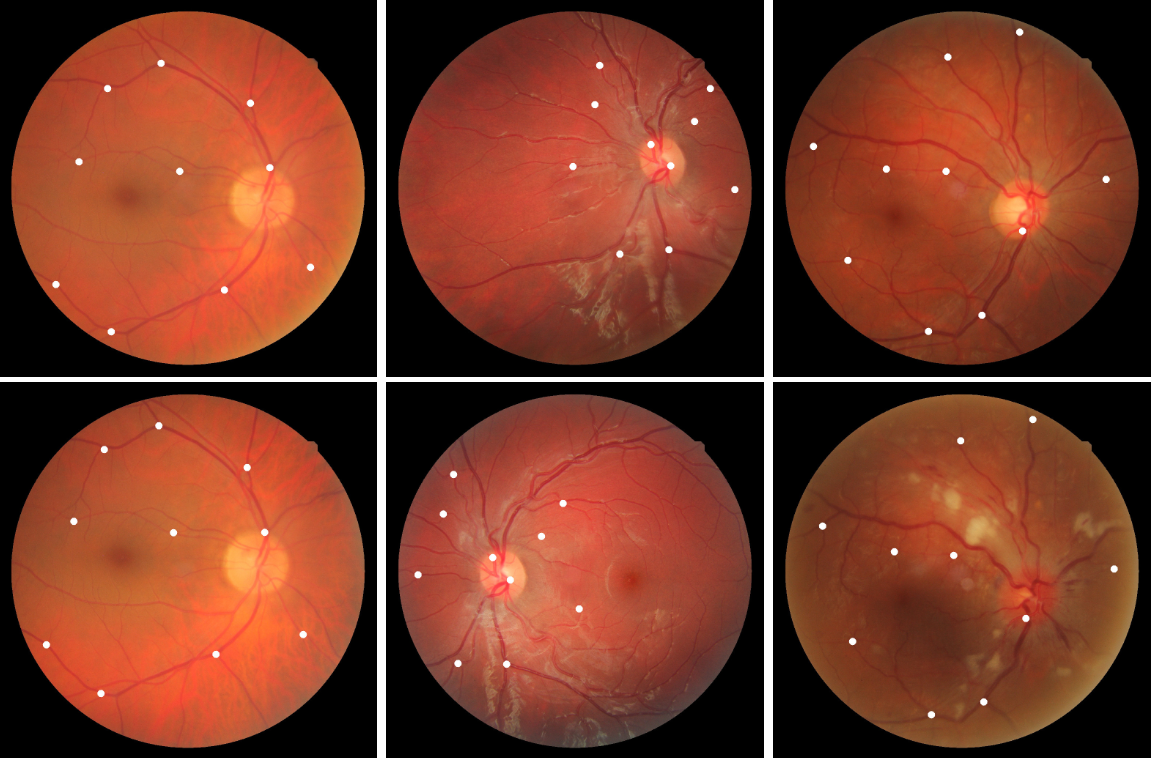
\includegraphics[width=0.8\textwidth]{imaxes/fire-ej.png}
    \caption{Exemplo de imaxes do conxunto de datos FIRE \cite{FIRE} cos puntos de control indicados. De esquerda a dereita, categorías \textit{\textsf{S}}, \textit{\textsf{P}}, \textit{\textsf{A}} .}
    \label{fig:fire_ej}
\end{figure}

\subsection{RFMID}
\label{subsec:RFMID}

O conxunto de datos RFMiD \cite{RFMiD} proporciona 3200 imaxes de fondo de ollo en cor con resolución 1712x1712, etiquetadas según se teñen algunha anomalía ou non. 
Tamén proporciona etiquetas para 45 diferentes anomalías anotadas por expertos.

Para utilizalo neste traballo, seleccionamos unha submostra e xeramos transformacións aleatorias. Gardamos as imaxes orixinais e as transformadas así como as matrices de transformación asociadas para a posterior avaliación.
Tamén se divide entre transfomacións de cor e de xeometría.

% \dots preguntar David


\subsection{Diferencias entre os datasets}
\label{subsec:Diferencias entre os datasets}

Unha vantaxe de utilizar dous conxutos de datos diferentes é que cada un deles ten características únicas que permiten avaliar o modelo en diferentes contextos.
A principal diferencia é que RMiFD é un conxunto de datos sintético, no cal non introducimos diferenzas de cor e sempre teñen unha superposición do 100\%, polo que o único que se avalia é a capacidade do modelo para realizar os rexistros xeométricos.
Polo contrario, FIRE é un conxunto de datos real, no cal existen cambios na iluminación, contraste, superposición e demais diferencias visuais, polo que se avalía a capacidade do modelo para realizar rexistros en condicións moito máis adversas.

\section{Métodos de Avaliación}
\label{sec:Métodos de Avaliación}

A evaluación divídese en dous tipos: a avaliación cualitativa, na cal analízanse os resultados de forma visual,
 e a avaliación cuantitativa, na cal se utilizan métricas numéricas para comparar os resultados en base a un criterio obxetivo.

 Ambas avaliacións son necesarias para obter unha visión completa da calidade do rexistro, xa que a avaliación cuantitativa pode non ser suficiente para detectar problemas visuais que non se reflictan nas métricas.

 \subsection{Avaliación Cuantitativa}
 \label{subsec:Avaliación Cuantitativa}
 
 Utilizamos como método de evaluación cuantitativa o proposto por FIRE \cite{FIRE}
 xerando un gráfico onde o eixo x representa o valor do límite de erro e o eixo y mostra a porcentaxe de pares de imaxes que foron rexistrados con éxito para cada límite de erro.
 
 O error de rexistro calcúlase ca distancia media entre os puntos correspondentes na imaxe fixa e móbil (cj, rj).
 Cando o erro de rexistro entre un par de imaxes está por debaixo do límite, considérase que o rexistro foi exitoso e viceversa. Isto dá lugar a unha curva monótona e continua que reflicte a relación entre a taxa de éxito e a precisión obxectivo, evitando así a necesidade de establecer un limiar arbitrario. 
 Estes gráficos utilízanse para ilustrar a precisión do rexistro tanto para casos individuais (onde se utilizan o porcentaxe de parellas de puntos rexistrados con éxito)
  como para o conxunto completo de datos.
 
Esta métrica facilita a comparación entre distintos métodos competidores e permite seleccionar o máis axeitado segundo a precisión desexada.
 
 Mentres que FIRE xa provee os puntos de referencia para a avaliación, RFMID non o fai.
 Polo tanto, para RFMID, utilizamos o mesmo método de avaliación, pero xerándo os puntos manualmente de forma que cubran o interior da máscara da imaxe fixa (separados por 50 píxeles entre si).
 
 \begin{figure}[ht]
    \centering
    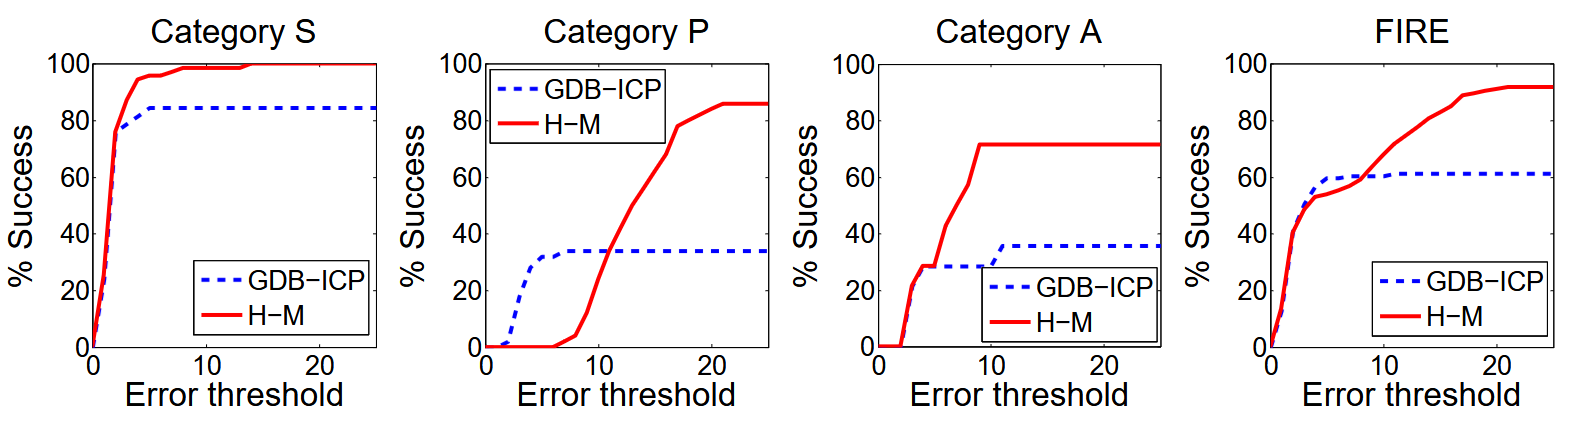
\includegraphics[width=0.8\textwidth]{imaxes/fire_aval.png}
    \caption{Gráfico de avaliación FIRE, \cite{FIRE}}
    \label{fig:fire_aval}
\end{figure}

Nalgúns casos, utilizaremos a distancia media entre os puntos correspondentes como métrica adicional para avaliar a calidade do rexistro, xa que a taxa de éxito pode non ser suficiente para detectar os cambios.

\subsection{Avaliación Cualitativa}
\label{subsec:Avaliación Cualitativa}

No caso deste traballo, a avaliación cualitativa cobra gran importancia, xa que na cuantitativa so se está a comparar sobre un número reducido de puntos en cada parexa de imaxes.
A avaliación visual permite detectar problemas que non se reflictan nas métricas cuantitativas, como artefactos visuais ou deformacións non desexadas, 
especialmente en rexistros que teñen deformacións locais que poden non coincidir con ningún punto.

No caso do dataset FIRE \cite{FIRE}, a avaliación visual é especialmente relevante, xa que tan só se proporcionan 10 puntos de referencia por imaxe, que poden non ser suficientes para avaliar a calidade do rexistro en moitas zonas da imaxe.
Xa que en RFMID \cite{RFMiD} utilízanse puntos de referencia xerados manualmente que cubren toda a imaxe, a avaliación visual é algo menos relevante, xa que é máis probable que unha deformación local incorrecta sexa detectada por algún punto e se vexa reflexado nas métricas.

\section{Proceso de Rexistro}
\label{sec:Proceso de Rexistro}

Inicializase a rede, ca arquitectura modificada nas capas de entrada e saída 
(orixinalmente [3, 256, 256, 256, 3], agora [2, 256, 256, 256, 2]) 
e o resto de parámetros relevantes (función de activación, optimizador, métrica de loss, termos de regularización, etc).

A inicialización dos pesos da rede é especialmente relevante no caso da función de activación SIREN, que é sensible a valores iniciais.
Tamén se xera un tensor de coordenadas inicial que contén todas as coordenadas dentro da máscara da imaxen fixa.

Cando comeza o adestramento por cada epoch repítese o seguinte proceso:

Mostreanse "batch size" puntos no tensor de coordenadas orixinal e estos pásanse pola rede, 
a cal devolve a transformación que predice para esas coordenadas.
A continuación, aplicase esta transformación e calculase o loss entre a imaxe móbil transformada e a imaxe fixa.
O valor de loss axústase según os termos de regularización usados, e finalmente realízase a retropropagación para actualizar os pesos da rede.

O proceso de mostraxe pode ser aleatorio ou utilizando unha estratexia específica.

Cabe destacar que a tarefa de rexistro de pulmóns é diferente da de retinografías. O tamaño das deformacións é moito maior, así como o grado de superposición entre as imaxes.
Por este motivo, non podemos asumir que os parámetros óptimos para pulmóns sexan tamén os mellores para retinas.